%%%%%%%%%%%%%%%%%%%%%%%%%%%%%%%%%%%%%%%%%%%%%%%%%%%%%%%%%
%%%
%%%  Chapter 2
%%%  Robot Overview
%%%
%%%%%%%%%%%%%%%%%%%%%%%%%%%%%%%%%%%%%%%%%%%%%%%%%%%%%%%%%
Moonbot is the first version of a modular robot model for the Moonshot project, "Self Evolving AI Robot System for Lunar Exploration and Human Outpost Construction". The aimed technologies of this robot are self-reconfigurable and self-assembly abilities. 

Using the internal sensors between main body and modular legs, Moonbot autonomously performs a real-time self-recognition system to identify the locomotion style fitting with the configuration.\\

\begin{figure}[ht]
  \centering
  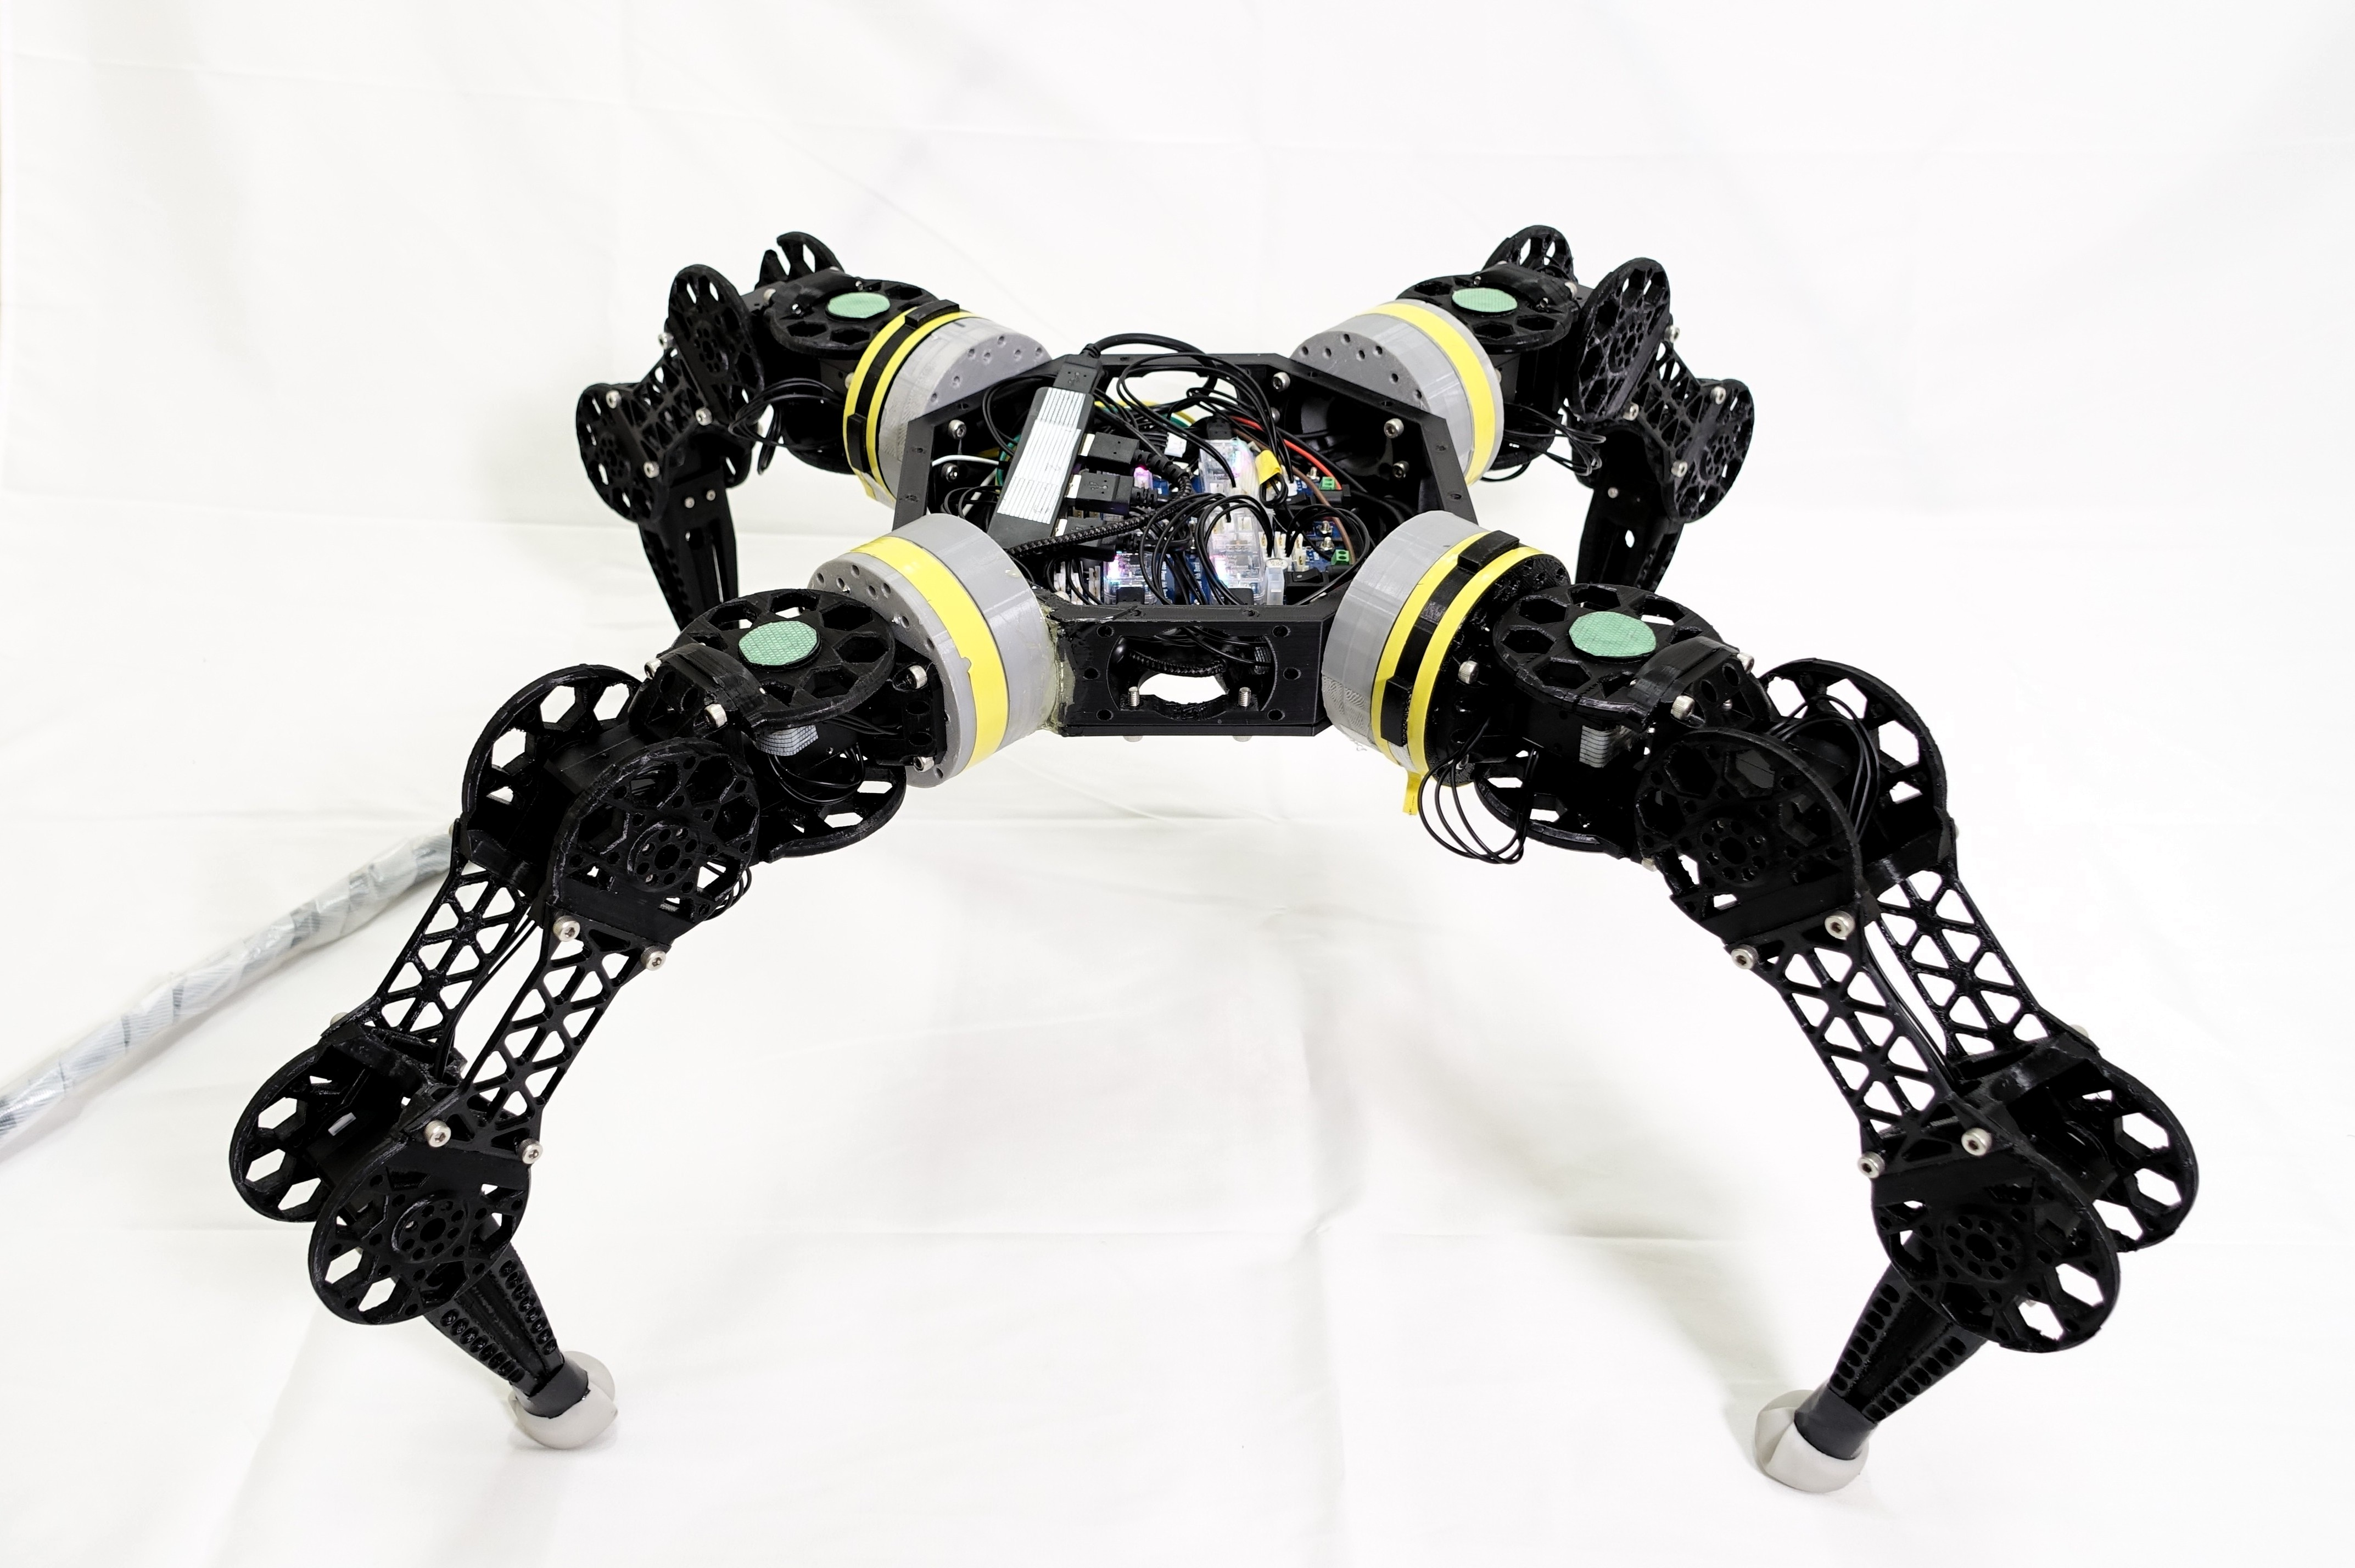
\includegraphics[width=100mm]{./fig/moonbot/moonbot1.jpg}
  \vspace{2mm}
  \caption{Moonbot with full configuration on the sand box.}\label{fig moonbot}
\end{figure}

%%%%% HARDWARE DESIGN %%%%%
\section{Hardware Design} % Find the exact material and add citation
The Moonbot's parts are mainly made of PLA (Ploylactic Acid) \cite{PLA}, 3D printed. The  Moonbot's components consist of central body and four leg modules. The legs are connected via magnetic connection. The communications of each leg and the computer transfer via pogo pin connector. In the this section, the mechanical design and electronic of Moonbot are explained

\subsection{Central Body}
The Moonbot's central body is 20x20 cm square shape. The total weight, including all electronic components, is 1.02 kilograms. On the body, there are four U2D2 and U2D2 hub, a USB communication converter for connecting with servo motors. This converter is available for various communication protocol, including 4-pin UART, 3-pin TTL, and 4-pin RS-485. In this time, 3-pin TTL is selected. At the bottom of the body, four ball casters are attached to support the locomotion style where the body of the robot lies on the floor. At each corner of the shape, four ports of magnetic connection are anchored.\\

\begin{figure}[t]
  \centering
  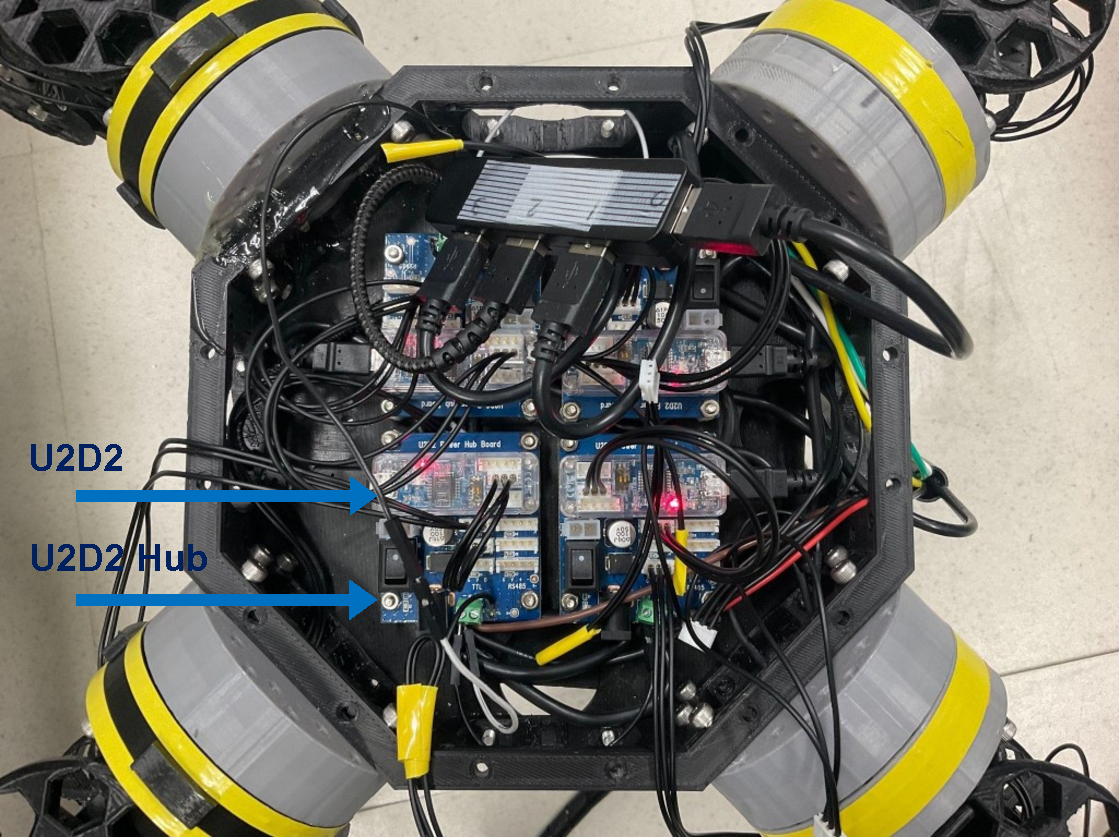
\includegraphics[width=90mm]{./fig/chap2/bodyelectronics.pdf}
  \vspace{2mm}
  \caption{Electronics components on the Moonbot center hub.}\label{electronics}
\end{figure}

\begin{figure}[t]
  \centering
  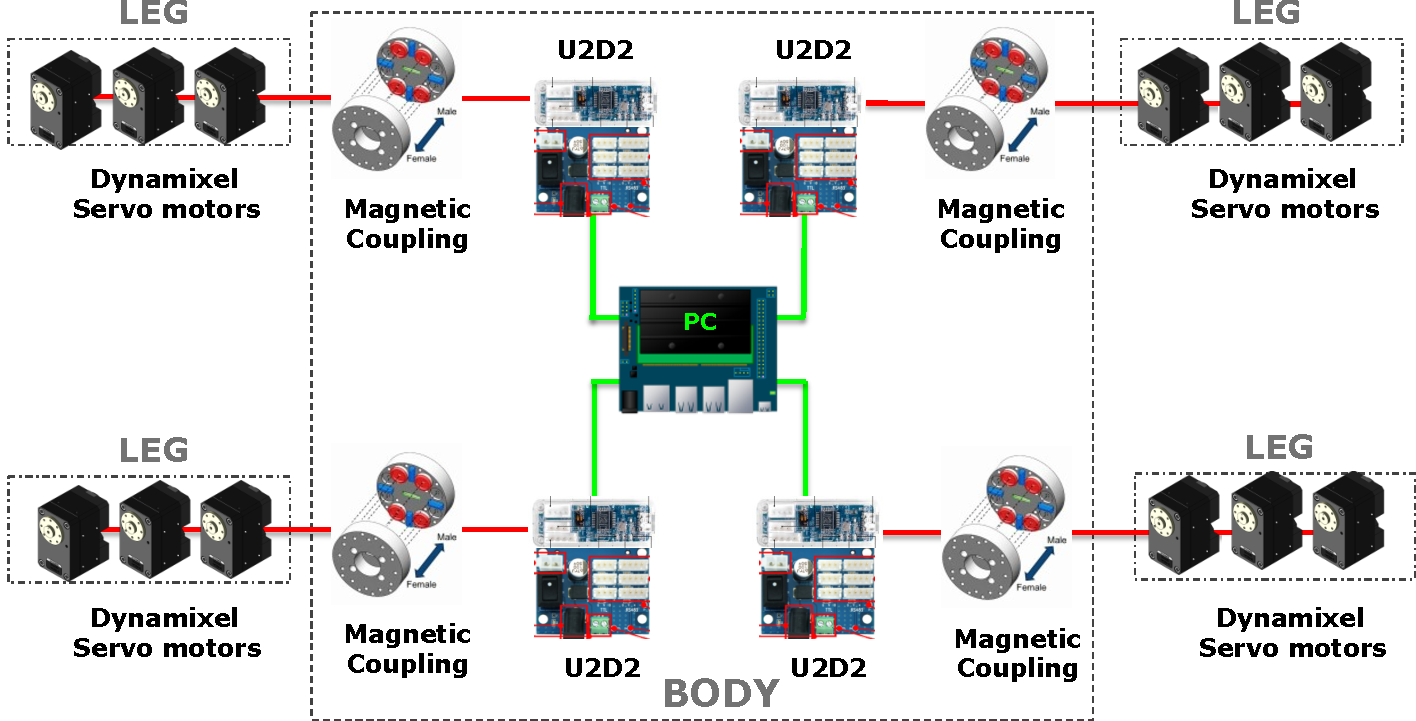
\includegraphics[width=140mm]{./fig/chap2/electronics_diagram.pdf}
  \vspace{2mm}
  \caption{Electronics components on the Moonbot center hub.}\label{electronics_diagram}
\end{figure}

\subsection{Magnetic Coupling}
Each of the legs is connected to the body via 8 pairs of circular Neodynium magnets, arranged in circular pattern as shown in as shown in \fig{magnet}. A piese of magnet has 180 grams of weight, 3 mm in height and 150 mm of diameter.

\begin{figure}[t]
  \centering
  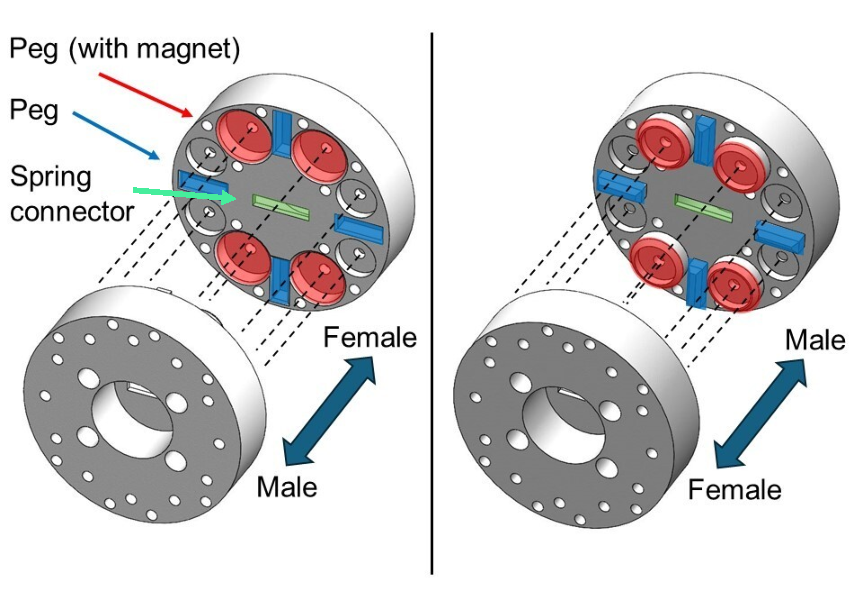
\includegraphics[width=110mm]{./fig/chap2/pogopin/connector2.pdf}
  \vspace{2mm}
  \caption{Magnetic connector.}\label{magnet}
\end{figure}

In addition to the magnetic coupling, the electronics connections between the body and the legs are facilitated by pogo pins. Pogo pins, also known as spring-loaded pins, provide a reliable electrical connection between two components while allowing for movement and flexibility. This spring loaded connector is attached at the center of the magnetics connector of each module as shown in \fig{pogopin}\\

\begin{figure}[h]
  \centering
  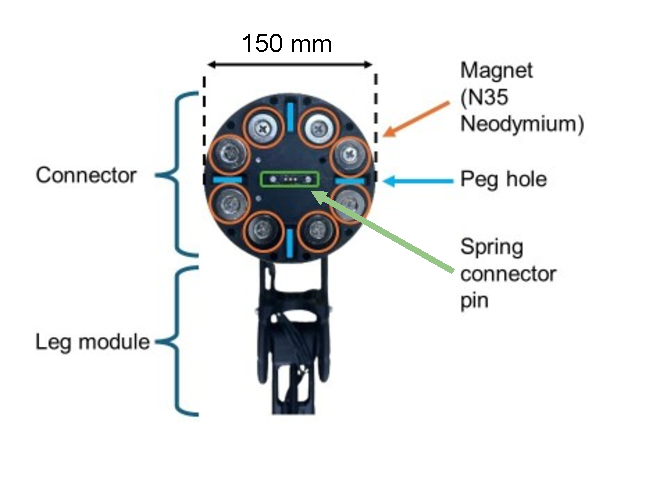
\includegraphics[width=120mm]{./fig/chap2/pogopin/connector.pdf}
  \vspace{2mm}
  \caption{Pogo pin connector located at the middle of magnetic coupling.}\label{pogopin}
\end{figure}

% \begin{figure}[t]
%     \begin{subfigure}{1.0\textwidth}
%      \begin{center}
%       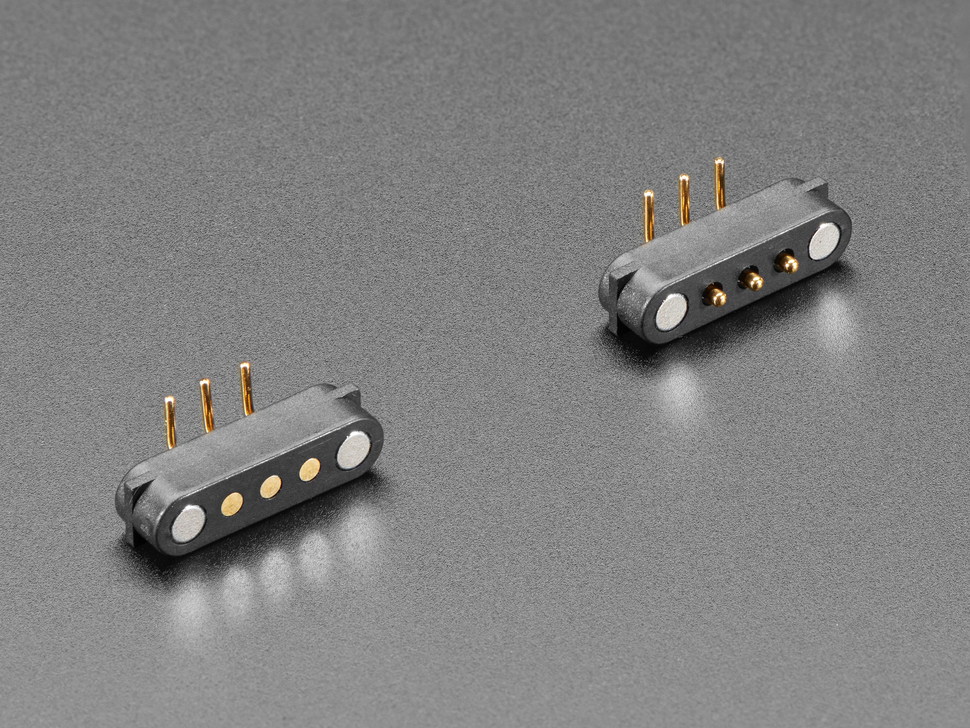
\includegraphics[height=30mm]{./fig/chap2/pogopin/pogopin3pin.jpg}
%     \caption{Three contact pins connector}\label{pogopin1}
%      \end{center}
%     \end{subfigure}
    
%     \begin{subfigure}{1.0\textwidth}
%      \begin{center}
%       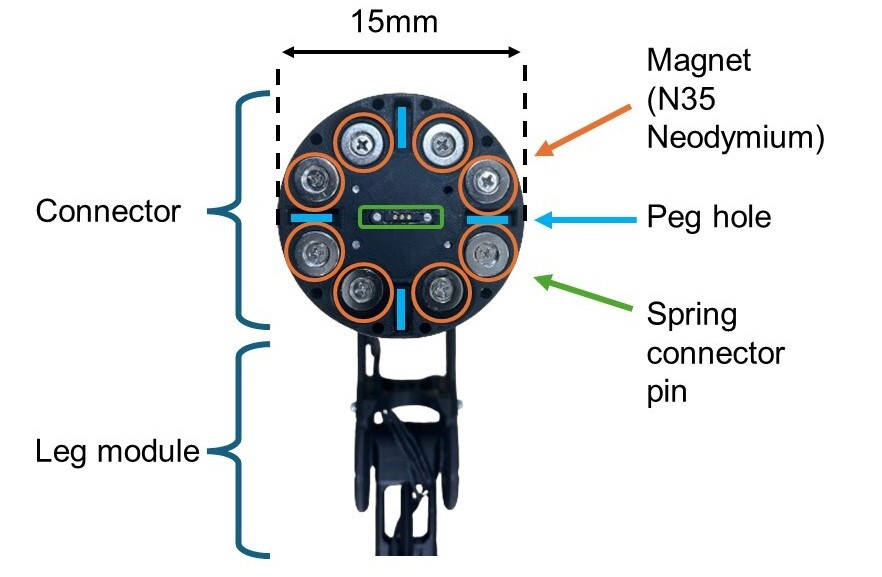
\includegraphics[height=70mm]{./fig/chap2/pogopin/connector.jpg}
%     \caption{Pogopin of the leg module}\label{pogopin2}
%     \end{center}
%     \end{subfigure}
%     \vspace{2mm}
%     \caption{Overview of magnet-based connector}
%     \label{pogopin}
% \end{figure}

\subsection{Modular Leg Modules}
Moonbot consists of four modular legs, utilizing a yaw-pitch-pitch configuration. Each of the leg has 530 grams with a small cylindrical end effector.The lengths of each link of the leg are shown in Table \ref{moonbot params}

\vspace{\baselineskip}
\begin{table}[h]
  \centering
    \caption{Moonbot's leg parameters.}
     \begin{tabular}{rrr} 
     \bhline{1.2pt}
      \multicolumn{1}{c}{Link's name}&\multicolumn{1}{c}{Length [mm]} \\
      % \multicolumn{1}{c}{of data}&\multicolumn{1}{c}{[mm]}&\multicolumn{1}{c}{±std [mm] } \\
      \hline
      Coxa	&	64.55		\\
      Femur	&	129.0	\\
      Tibia	&	156.0	\\
     \bhline{1.2pt}
    \end{tabular}
    \vspace{2mm}
    \label{moonbot params}
\end{table}
% \vspace{\baselineskip}

\begin{figure}[h]
  \centering
  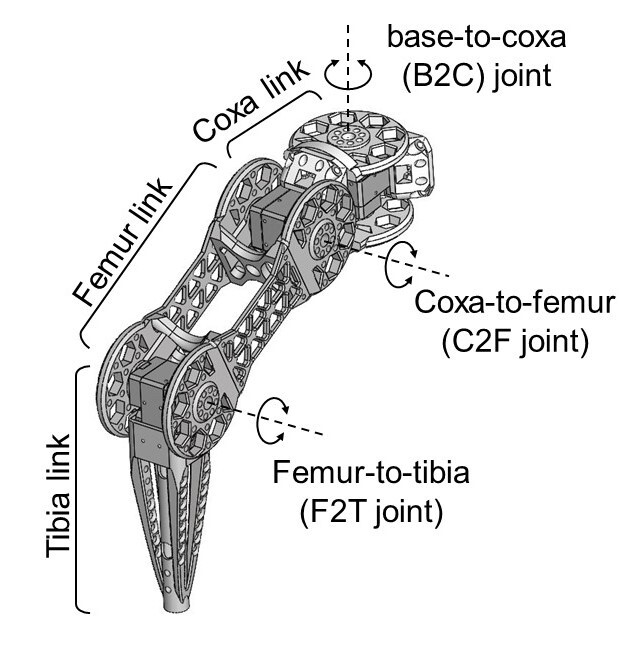
\includegraphics[width=90mm]{./fig/leg_configuration/CAD.jpg}
  \vspace{2mm}
  \caption{Moonbot's modular legs.}\label{modules}
\end{figure}

%%%%% SERVO %%%%%
\subsection{Joints' Actuator: Dynamixel}
Dynamixel is a brand of high-performance smart servos developed by ROBOTIS~\cite{robotis}. These servos are widely used in robotics applications due to their precision, durability, and advanced features. Dynamixel servos are known for their ability to provide position, velocity, and torque control, as well as various feedback mechanisms.

The joints of the Moonbot is moved by Dynamixel XM430-350-T, utilizing a 3-pin TTL communication protocol, Moonbot can generate trajectories with precise position control. The specification of this servo is shown below\\

\begin{figure}[t]
  \centering
  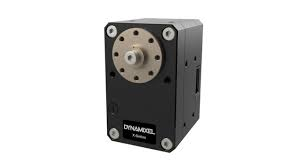
\includegraphics[width=90mm]{./fig/chap2/dxl.jpeg}
  \vspace{2mm}
  \caption{Dynamixel servo motor, model XM430-W350-T.}\label{DXL}
\end{figure}
\smallskip
\begin{table}[t]
    \centering
    \caption{Dynamixel XM430-W350-T Specifications.}
    \label{dynamixel_spec}
    \begin{tabular}{|l|l|}
        \hline
        \rowcolor[HTML]{EFEFEF}
        \multicolumn{2}{|c|}{\cellcolor[HTML]{EFEFEF}\textbf{Specifications}} \\ \hline
        \textbf{Parameter} & \textbf{Value} \\ \hline
        Speed & 46 RPM \\ \hline
        Torque & 4.1 N$\cdot$m  \\ \hline
        Size & 33.5$\times$46.5$\times$34.0 mm \\ \hline
        Mass & 82 g \\ \hline
    \end{tabular}
\end{table}
\smallskip
%%%%% SERVO %%%%%

%%%%% HARDWARE DESIGN %%%%%
%%% EOF %%%